\documentclass[12pt]{article}
\usepackage[margin=1in]{geometry}
\usepackage[parfill]{parskip}
\usepackage{newtxtext}
\usepackage{booktabs}
\usepackage{fancyvrb}
\usepackage{graphicx}

\title{DMA \\
\large 18-1 ECE 322 Computer Organization, Lab 08}
\author{Hansung Kim \\ 2014-16824}
\date{}

\begin{document}
\maketitle

\section{Introduction}
Implement a DMA controller on top of the previous CPU implementation.
Learn how CPU cooperates with DMA to achieve better performance.

\section{Design}

The key point of this design is the use of a signal called
\verb|d_cache_busy| that indicates whether the cache is occupying the
data and address bus, i.e. handling cache miss.  The addition of this
single signal simplifies the logic of granting of the bus to the DMA.

\subsection{Bus grant and reclaim}

The CPU can grant the bus access to the DMA controller whenever the
cache is not handling miss, i.e. \verb|d_cache_busy == 0|.
Conversely, if the DMA controller stops requesting for the bus, it is
guaranteed that the bus is vacant and the CPU can reclaim the access
immediately.  Therefore, the code for the bus grant and reclaim logic
is simply as follows:

\begin{figure}[ht]
  \centering
  \begin{BVerbatim}
  if (bus_request && !d_cache_busy) begin
     bus_granted <= 1;
  end

  if (!bus_request) begin
     bus_granted <= 0;
  end
  \end{BVerbatim}
  \caption{Bus grant and reclaim logic using \texttt{d\_cache\_busy}}
  \label{fig:bus-logic}
\end{figure}

where \verb|d_cache_busy| is produced by testing if the cache is being
read or write but its value is not ready, i.e.  \texttt{(d\_readC OR
  d\_writeC) \&\& !d\_readyC}.

\subsection{Cycle stealing}
The DMA cycle stealing of the CPU can be implemented easily with
little modification.  After each memory write of 4 words, the DMA
controller sets \verb|bus_request| to zero for exactly one cycle.
This causes the CPU to retry any currently blocked memory operation in
that single cycle.  If there were any, the operation will set
\verb|d_cache_busy| on, delaying the \verb|bus_granted| to go up until
the operation is finished.  If there were no blocked memory operation,
the logic in Figure \ref{fig:bus-logic} would set \verb|bus_granted|
back on immediately.  Therefore, the Figure \ref{fig:bus-logic} logic
is capable of handling cycle stealing by itself.

\section{Implementation}

\subsection{DMA module}
A new module called DMA (\verb|dma.v|) is created to implement the
DMA-side transaction logic.  The logic is implemented by the use of
\verb|cmd|, \verb|BG|, \verb|offset| and \verb|doneM| signals.

\begin{enumerate}
\item Upon the CPU interrupt from the device, the CPU sets \verb|cmd|
  with non-zero command signals. The DMA controller listens on this
  signal on each clock edge, and turns \verb|BR| to one.  It also
  caches the \verb|cmd| to its internal register to keep it alive
  during the transaction.
\item The CPU sets \verb|BG| to on whenever its memory operation that
  had been running at the point of interrupt is finished.  Upon detecting
  this \verb|BG|, the DMA
  controller issues memory write using the designated address and length
  in the \verb|cmd|.
\item The controller is notified of the write finish via \verb|doneM|
  signal from the memory module.  Upon each \verb|doneM|, the
  controller increments the \verb|offset| counter held in an internal
  register.  If the offset matches \verb|len - 1|, the controller
  determines the data write is over, and resets both \verb|offset| and
  \verb|BR| to zero.
\item The clearing of \verb|BR| triggers the CPU to retry its blocking
  memory operation and resume the pipeline.  Finally, the controller
  sets the interrupt signal for 1 cycle and goes back to listening on
  \verb|cmd|.
\end{enumerate}

\subsubsection{Modification for cycle stealing}
To implement the cycle stealing, the step 3 of the above process
should be modified to reset \verb|BR| and set it back on immediately,
for every memory write finish (\verb|doneM|).  This causes the
CPU-side logic (\verb|datapath.v|) to automatically retry its blocking
memory operation, as in step 4, upon every 4-word memory write.  It
will subsequently set \verb|BG| to on, causing the DMA to proceed for
remaining data writes.  As this process is made possible by only
changing the set and reset timing of the \verb|BR| signal, no change
in the CPU-side logic is required.

\subsection{Changes to the datapath}
The bus granting and reclaiming logic (Figure \ref{fig:bus-logic}),
which is the CPU-side handling of the transaction, is implemented in
the datapath module (\verb|datapath.v|) with some additional logic to
construct the command.  Also, the stalling of the pipeline upon bus
request is implemented in the hazard unit submodule
(\verb|hazard_unit.v|).

\subsubsection{Command signal structure}
The DMA command is simply implemented as a concatenation of the
address of the memory to write and the length of the external data.
In other words, it is a 2-word vector whose \verb|cmd[31:16]| is
\verb|addr[15:0]|, and \verb|cmd[15:0]| is \verb|len[15:0]|.

\subsubsection{Changes to the hazard unit}
The hazard unit stalls the entire pipeline on \verb|d_cache_busy|.
This single check happens to be enough for handling both the D-cache
miss (for ordinary load/store instructions) and the bus sharing with
DMA, since \verb|d_cache_busy| will be set to zero in both cases.
Thus, the hazard unit does not require any modification from the cache
implementation (aside from the variable renaming).

\subsection{Changes to the cache}
The cache is modified to not issue any memory read/write when the bus
is granted.  Its ``ready'' state should also remain false for the
whole time span of bus grant.  Thus, the \verb|readM|, \verb|writeM|
and \verb|readyC| signal is additionally logical-ANDed with
\verb|!bus_granted|, which effectively no-ops the cache operation when
the bus is granted to the DMA.

\subsection{Waveform}

The waveform plot of the related signals is shown in Figure
\ref{fig:waveform1} and \ref{fig:waveform2}.  Figure
\ref{fig:waveform1} shows the delayed bus grant due to the memory
operation that was running in the CPU (\verb|writeC| and \verb|writeM|
due to D-cache write-through) at the point of the DMA bus request.
Figure \ref{fig:waveform2} shows the successful cycle stealing of the
CPU, where it resumes its pending memory operation in the middle of
the DMA operation (\verb|writeC| and \verb|writeM| of the D-cache),
which was triggered by the DMA temporarily disabling its bus request.

From the \verb|pc| signal at the top, it can also be confirmed that
other memory-independent operations proceed to run in the pipeline
during the DMA operation.

To confirm that the DMA had actually written to the memory, the
\verb|d_dma_mem| signal at the bottom shows the memory content at the
designated address (\verb|memory[0x01f4]|), which indeed changes to
the \verb|edata| value immediately after the first DMA write.

\begin{figure}[!ht]
  \centering
  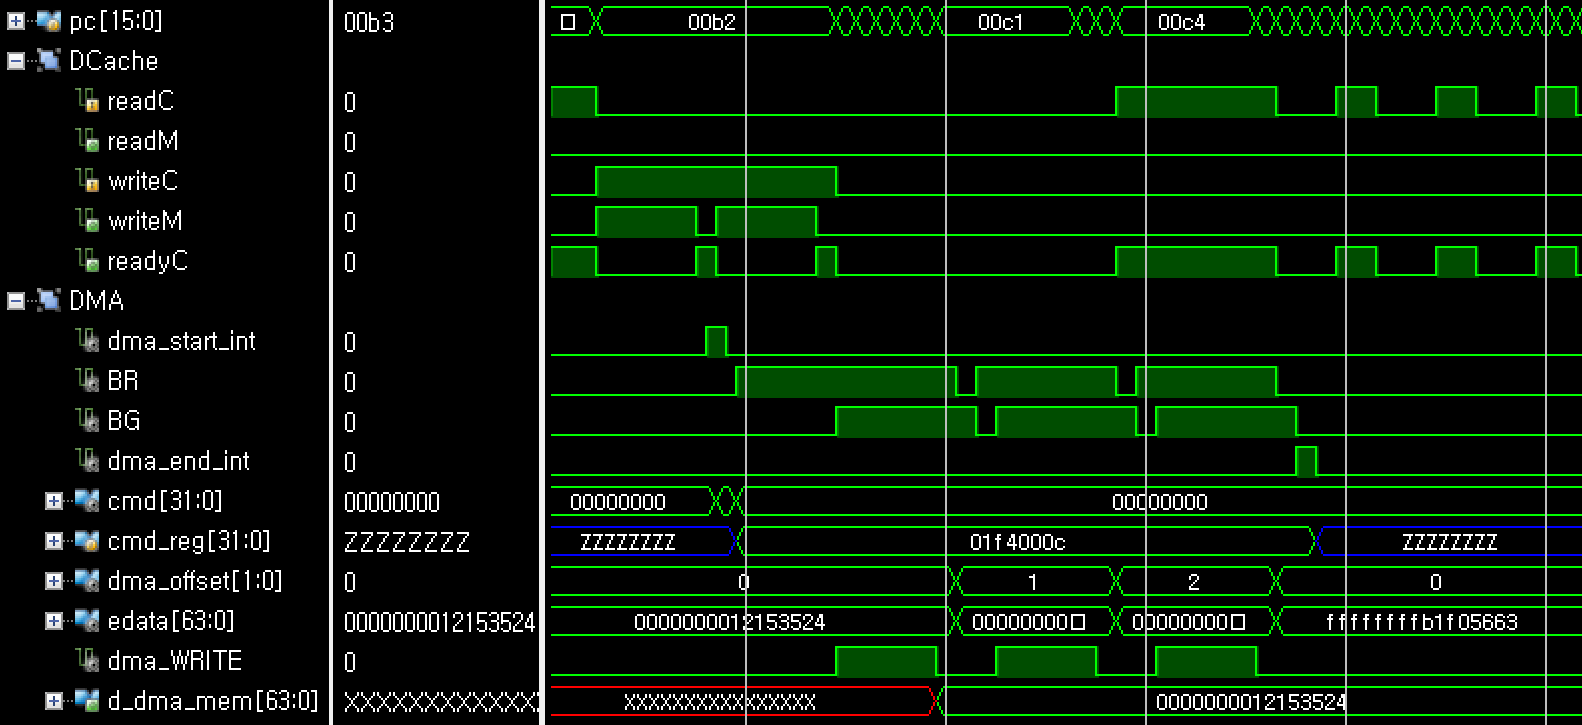
\includegraphics[scale=0.8]{dma_cyclesteal_1}
  \caption{Waveform of the DMA and D-cache signals with no successful cycle stealing}
  \label{fig:waveform1}
\end{figure}

\begin{figure}[!ht]
  \centering
  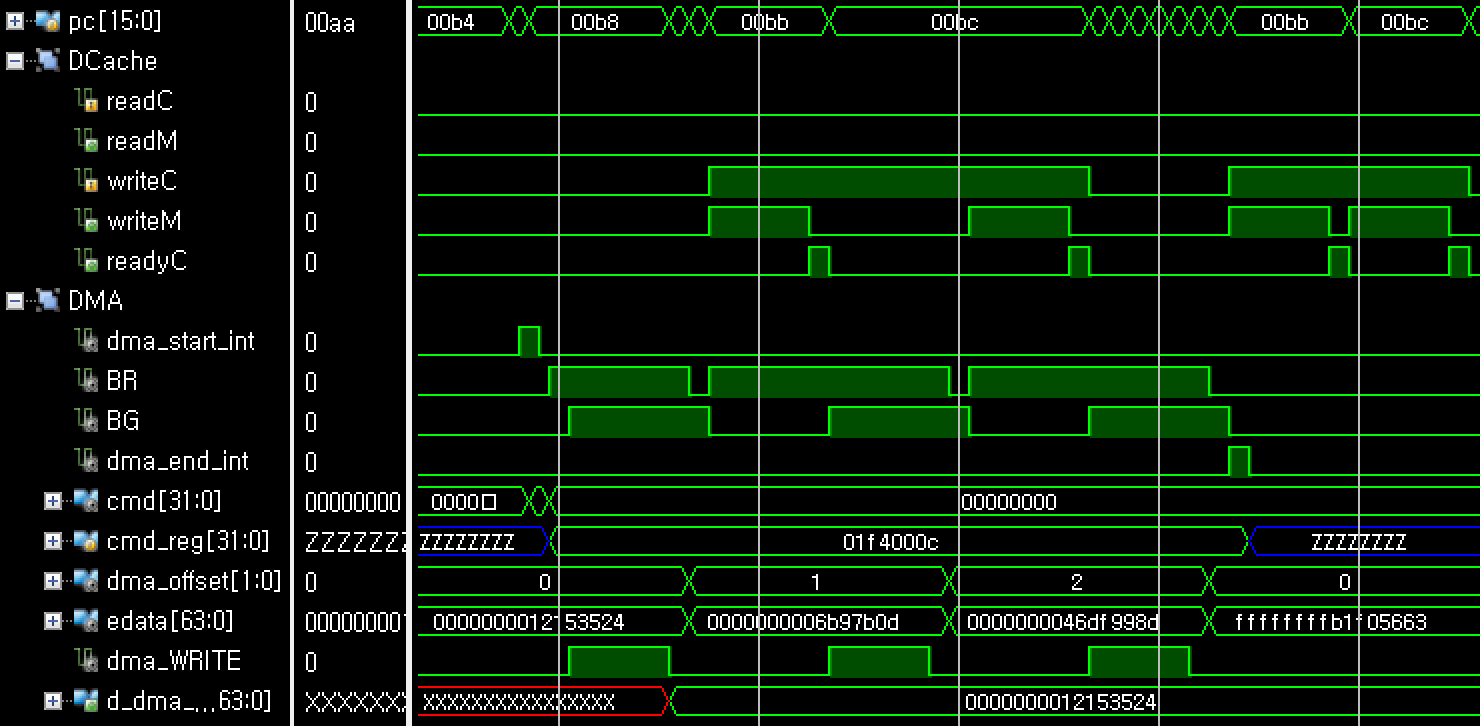
\includegraphics[scale=0.8]{dma_cyclesteal_2}
  \caption{Waveform of the DMA and D-cache signals with two successful cycle stealing}
  \label{fig:waveform2}
\end{figure}

\section{Discussion}
A simple DMA controller along with cycle stealing could be
successfully implemented.  Compared to the previous version, the
number of clock cycles to finish the testbench increased from 2796 to
2802, which is natural considering the additional latency caused by
DMA occupying the memory bus and preventing the pipeline to proceeed.

A quick test showed that the implementation without cycle stealing
shows the clock cycles of 2806.  The performance increase due to cycle
stealing is marginal.  However, cycle stealing has the advantage that
it does not leave the CPU completely unresponsive during the device
communication, which could be a major problem for slow devices that
require long I/O time.

\section{Conclusion}
Successfully implemented a DMA controller on top of the previous CPU
implementation.  Learned how CPU cooperates with DMA to achieve better
performance.

\end{document}